\subsection{Blazemark}
Blazemark is a benchmark suite provided by Blaze to compare the performance of Blaze with other linear algebra libraries.

\vspace{\baselineskip}	
\section{Parallelization in Blaze}
Depending on the operation and the size of operands, this assignment could be parallelized through four different backends, namely, HPX, OpenMP\cite{dagum1998openmp}, C++ threads, and Boost\cite{Boost}. 

Blaze offers parallelization through 4 different backends
\vspace{\baselineskip}	
\subsection{Implementation of HPX Backend}
As stated earlier, as an ET-based library, blaze performs the calculations when an expression is assigned to a target, which is implemented through the \textit{blaze::Assign} function
Different backends are implemented in Blaze through a for-loop in which at each iteration a section of the vector or matrix is selected and the result of the operation is assigned to the corresponding section of the result. 
Each backend uses their own method for parallelizing this for loop. For HPX backend the HPX \textit{parallel::for\textunderscore loop} is used for this purpose. 
Listing~\ref{hpx_backend} shows the modified implementation of HPX backend in Blaze.

\begin{lstlisting}[float,floatplacement=H,caption= {Previous implementation of Assign function for HPX backend in Blaze.}, label={old_hpx_backend}]
template< typename MT1   // Type of the left-hand side dense matrix
, bool SO1       // Storage order of the left-hand side dense matrix
, typename MT2   // Type of the right-hand side dense matrix
, bool SO2       // Storage order of the right-hand side dense matrix
, typename OP >  // Type of the assignment operation
void hpxAssign( DenseMatrix<MT1,SO1>& lhs, const DenseMatrix<MT2,SO2>& rhs, OP op )
{
using hpx::parallel::for_loop;
using hpx::parallel::execution::par;

BLAZE_FUNCTION_TRACE;

using ET1 = ElementType_t<MT1>;
using ET2 = ElementType_t<MT2>;

constexpr bool simdEnabled( MT1::simdEnabled && MT2::simdEnabled && IsSIMDCombinable_v<ET1,ET2> );
constexpr size_t SIMDSIZE( SIMDTrait< ElementType_t<MT1> >::size );

const bool lhsAligned( (~lhs).isAligned() );
const bool rhsAligned( (~rhs).isAligned() );

const size_t threads    ( getNumThreads() );
const ThreadMapping threadmap( createThreadMapping( threads, ~rhs ) );

const size_t addon1     ( ( ( (~rhs).rows() % threadmap.first ) != 0UL )? 1UL : 0UL );
const size_t equalShare1( (~rhs).rows() / threadmap.first + addon1 );
const size_t rest1      ( equalShare1 & ( SIMDSIZE - 1UL ) );
const size_t rowsPerThread( ( simdEnabled && rest1 )?( equalShare1 - rest1 + SIMDSIZE ):( equalShare1 ) );

const size_t addon2     ( ( ( (~rhs).columns() % threadmap.second ) != 0UL )? 1UL : 0UL );
const size_t equalShare2( (~rhs).columns() / threadmap.second + addon2 );
const size_t rest2      ( equalShare2 & ( SIMDSIZE - 1UL ) );
const size_t colsPerThread( ( simdEnabled && rest2 )?( equalShare2 - rest2 + SIMDSIZE ):( equalShare2 ) );

for_loop( par, size_t(0), threads, [&](int i)
{
const size_t row   ( ( i / threadmap.second ) * rowsPerThread );
const size_t column( ( i % threadmap.second ) * colsPerThread );

if( row >= (~rhs).rows() || column >= (~rhs).columns() )
return;

const size_t m( min( rowsPerThread, (~rhs).rows()    - row    ) );
const size_t n( min( colsPerThread, (~rhs).columns() - column ) );

if( simdEnabled && lhsAligned && rhsAligned ) {
auto       target( submatrix<aligned>( ~lhs, row, column, m, n ) );
const auto source( submatrix<aligned>( ~rhs, row, column, m, n ) );
op( target, source );
}
else if( simdEnabled && lhsAligned ) {
auto       target( submatrix<aligned>( ~lhs, row, column, m, n ) );
const auto source( submatrix<unaligned>( ~rhs, row, column, m, n ) );
op( target, source );
}
else if( simdEnabled && rhsAligned ) {
auto       target( submatrix<unaligned>( ~lhs, row, column, m, n ) );
const auto source( submatrix<aligned>( ~rhs, row, column, m, n ) );
op( target, source );
}
else {
auto       target( submatrix<unaligned>( ~lhs, row, column, m, n ) );
const auto source( submatrix<unaligned>( ~rhs, row, column, m, n ) );
op( target, source );
}
} );
}
\label{hpx_backend}
\end{lstlisting}

\begin{lstlisting}[float,floatplacement=H,caption= {New implementation of Assign function for HPX backend in Blaze.}, label={newd_hpx_backend}]
template< typename MT1   // Type of the left-hand side dense matrix
, bool SO1       // Storage order of the left-hand side dense matrix
, typename MT2   // Type of the right-hand side dense matrix
, bool SO2       // Storage order of the right-hand side dense matrix
, typename OP >  // Type of the assignment operation
void hpxAssign( DenseMatrix<MT1,SO1>& lhs, const DenseMatrix<MT2,SO2>& rhs, OP op )
{
using hpx::parallel::for_loop;
using hpx::parallel::execution::par;

BLAZE_FUNCTION_TRACE;

using ET1 = ElementType_t<MT1>;
using ET2 = ElementType_t<MT2>;

constexpr bool simdEnabled( MT1::simdEnabled && MT2::simdEnabled && IsSIMDCombinable_v<ET1,ET2> );
constexpr size_t SIMDSIZE( SIMDTrait< ElementType_t<MT1> >::size );

const bool lhsAligned( (~lhs).isAligned() );
const bool rhsAligned( (~rhs).isAligned() );

const size_t threads    ( getNumThreads() );
const size_t numRows ( min( static_cast<std::size_t>( BLAZE_HPX_MATRIX_BLOCK_SIZE_ROW ), (~rhs).rows() ) );
const size_t numCols ( min( static_cast<std::size_t>( BLAZE_HPX_MATRIX_BLOCK_SIZE_COLUMN ), (~rhs).columns() ) );

const size_t rest1      ( numRows & ( SIMDSIZE - 1UL ) );
const size_t rowsPerIter( ( simdEnabled && rest1 )?( numRows - rest1 + SIMDSIZE ):( numRows ) );
const size_t addon1     ( ( ( (~rhs).rows() % rowsPerIter ) != 0UL )? 1UL : 0UL );
const size_t equalShare1( (~rhs).rows() / rowsPerIter + addon1 );

const size_t rest2      ( numCols & ( SIMDSIZE - 1UL ) );
const size_t colsPerIter( ( simdEnabled && rest2 )?( numCols - rest2 + SIMDSIZE ):( numCols ) );
const size_t addon2     ( ( ( (~rhs).columns() % colsPerIter ) != 0UL )? 1UL : 0UL );
const size_t equalShare2( (~rhs).columns() / colsPerIter + addon2 );

hpx::parallel::execution::dynamic_chunk_size chunkSize ( BLAZE_HPX_MATRIX_CHUNK_SIZE );

for_loop( par.with( chunkSize ), size_t(0), equalShare1 * equalShare2, [&](int i)
{
const size_t row   ( ( i / equalShare2 ) * rowsPerIter );
const size_t column( ( i % equalShare2 ) * colsPerIter );

if( row >= (~rhs).rows() || column >= (~rhs).columns() )
return;

const size_t m( min( rowsPerIter, (~rhs).rows()    - row    ) );
const size_t n( min( colsPerIter, (~rhs).columns() - column ) );

if( simdEnabled && lhsAligned && rhsAligned ) {
auto       target( submatrix<aligned>( ~lhs, row, column, m, n ) );
const auto source( submatrix<aligned>( ~rhs, row, column, m, n ) );
op( target, source );
}
else if( simdEnabled && lhsAligned ) {
auto       target( submatrix<aligned>( ~lhs, row, column, m, n ) );
const auto source( submatrix<unaligned>( ~rhs, row, column, m, n ) );
op( target, source );
}
else if( simdEnabled && rhsAligned ) {
auto       target( submatrix<unaligned>( ~lhs, row, column, m, n ) );
const auto source( submatrix<aligned>( ~rhs, row, column, m, n ) );
op( target, source );
}
else {
auto       target( submatrix<unaligned>( ~lhs, row, column, m, n ) );
const auto source( submatrix<unaligned>( ~rhs, row, column, m, n ) );
op( target, source );
}
} );
}
\end{lstlisting}
\vspace{\baselineskip}	
\paragraph{HPX \textit{for\textunderscore loop}}
HPX \textit{for\textunderscore loop} takes an execution policy as first argument, which is set to \textit{dynamic\textunderscore chunk\textunderscore size} execution policy in case of HPX backend for Blaze.


\vspace{\baselineskip}	
\paragraph{Intuition}
It's hard to write a code that performs very well for all the applications, here we are interested to make the whole process as automatic as possible(without interference of a human expert), so that scientists could run their applications which highly depend on linear algebra libraries. 


To start, after collecting the data I tried to build a simple regression model to predict the performance based on the input features, only for the 'dmatdmatadd' benchmark. 

\vspace{\baselineskip}	
\section{Experiments}
In order to capture the relationship between number of cores, \textit{chunk\textunderscore{size}}, \textit{block\textunderscore{size}}, and the performance, we ran a series of experiments with different of these parameters and measured the number of floating point operations per second performed. 

For these experiments ,at the first step we selected the $DMatDMatADD$ benchmark which was implemented in Blazemark. $DMatDMatADD$ benchmark is a level 3 BLAS function to perform matrix-matrix addition in the form of $A=B+C$, where $A$, $B$, $C$ are square matrices of the same size. 

To avoid adding the scheduling overhead for small matrix sizes, Blaze uses a threshold to start parallelization, which is specific to the type of operation. For matrix-matrix addition, if the number of elements in the matrix is greater than 36100 elements(which is equivalent to a square matrix of size 190$\times$190) Blaze uses the configured backend to parallelize the assignment operation. For this reason, we start our experiments with matrix size of 200x200 and gradually increase the size to 1587$\times$1587. 


Figure~\ref{fig1} shows the results of running $DMatDMatADD$ benchmark for matrix sizes and number of cores listed in \tablename{name} based on grain size. Grain size 

\begin{figure}[H]
	\centering
	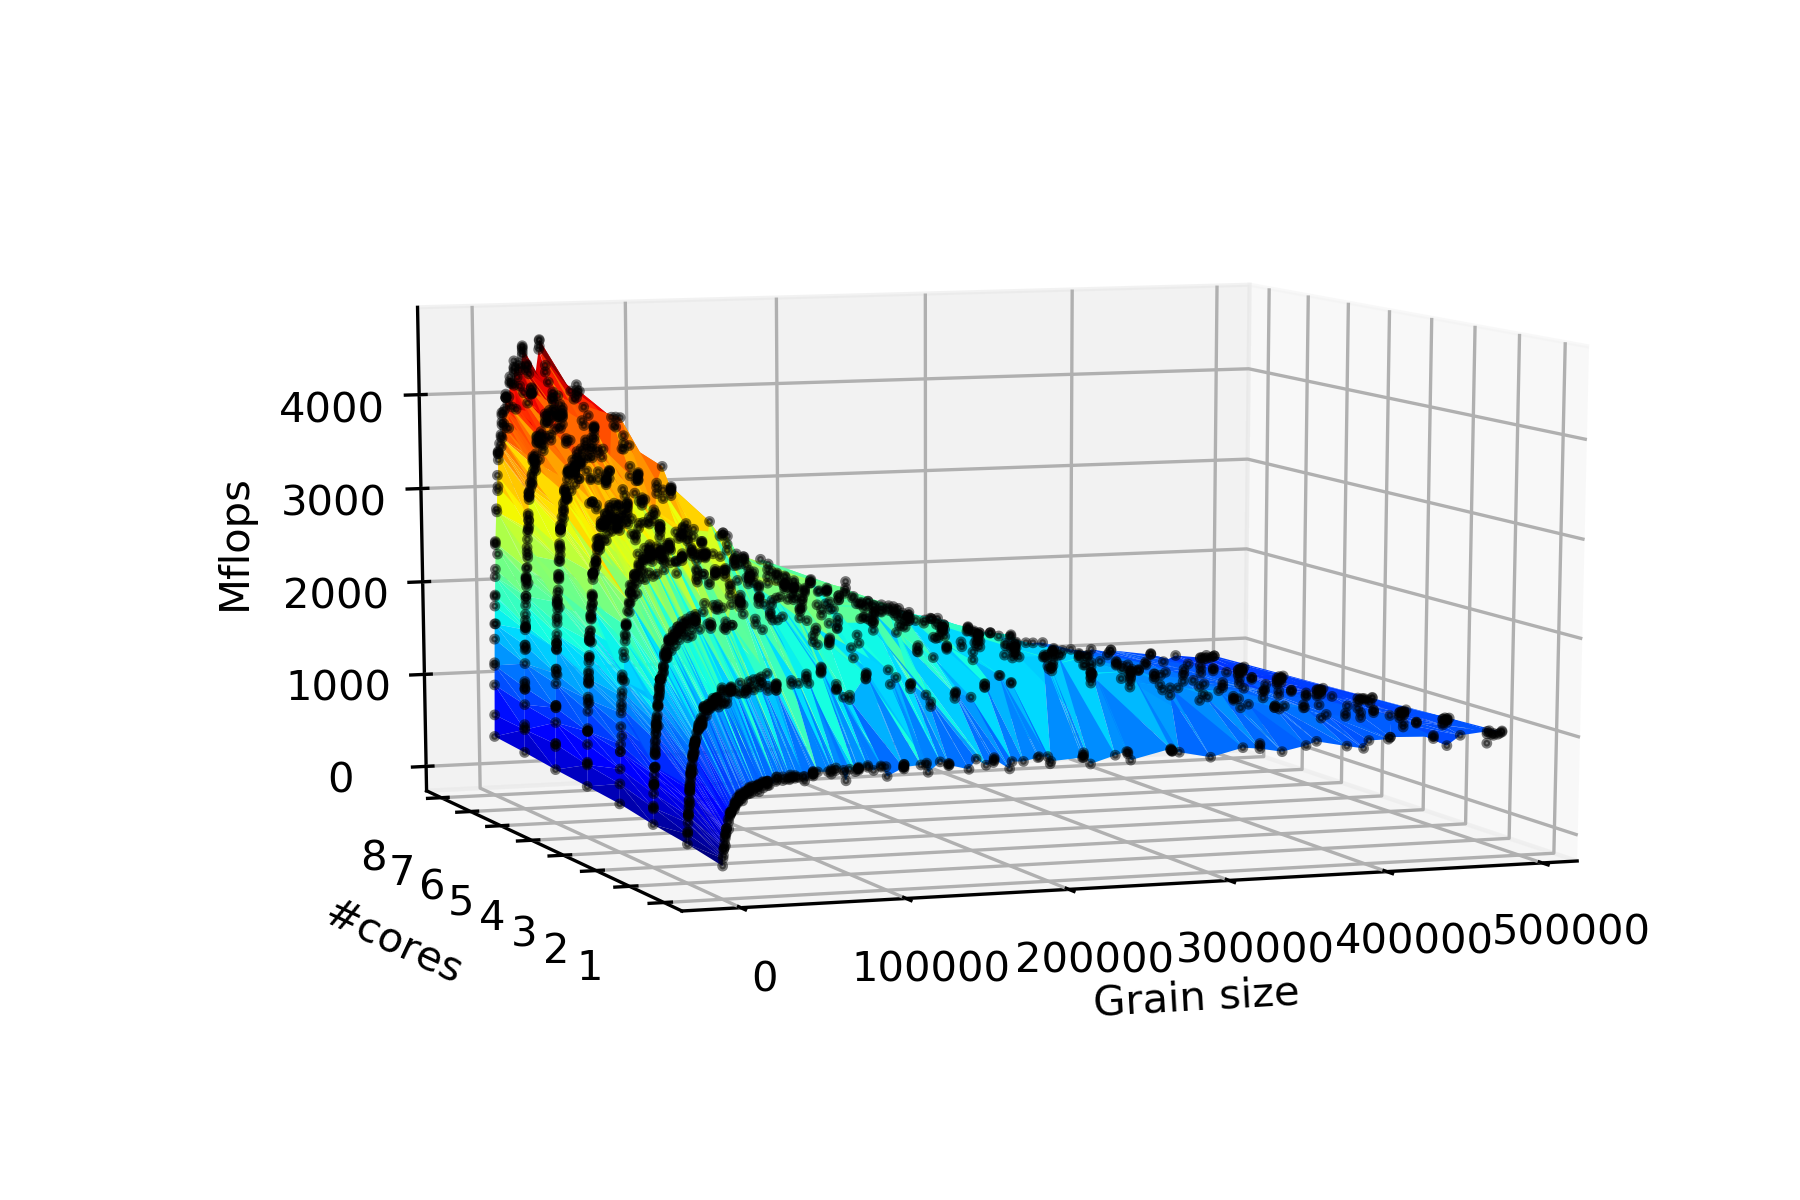
\includegraphics[width=1\linewidth]{images/fig2.png}
	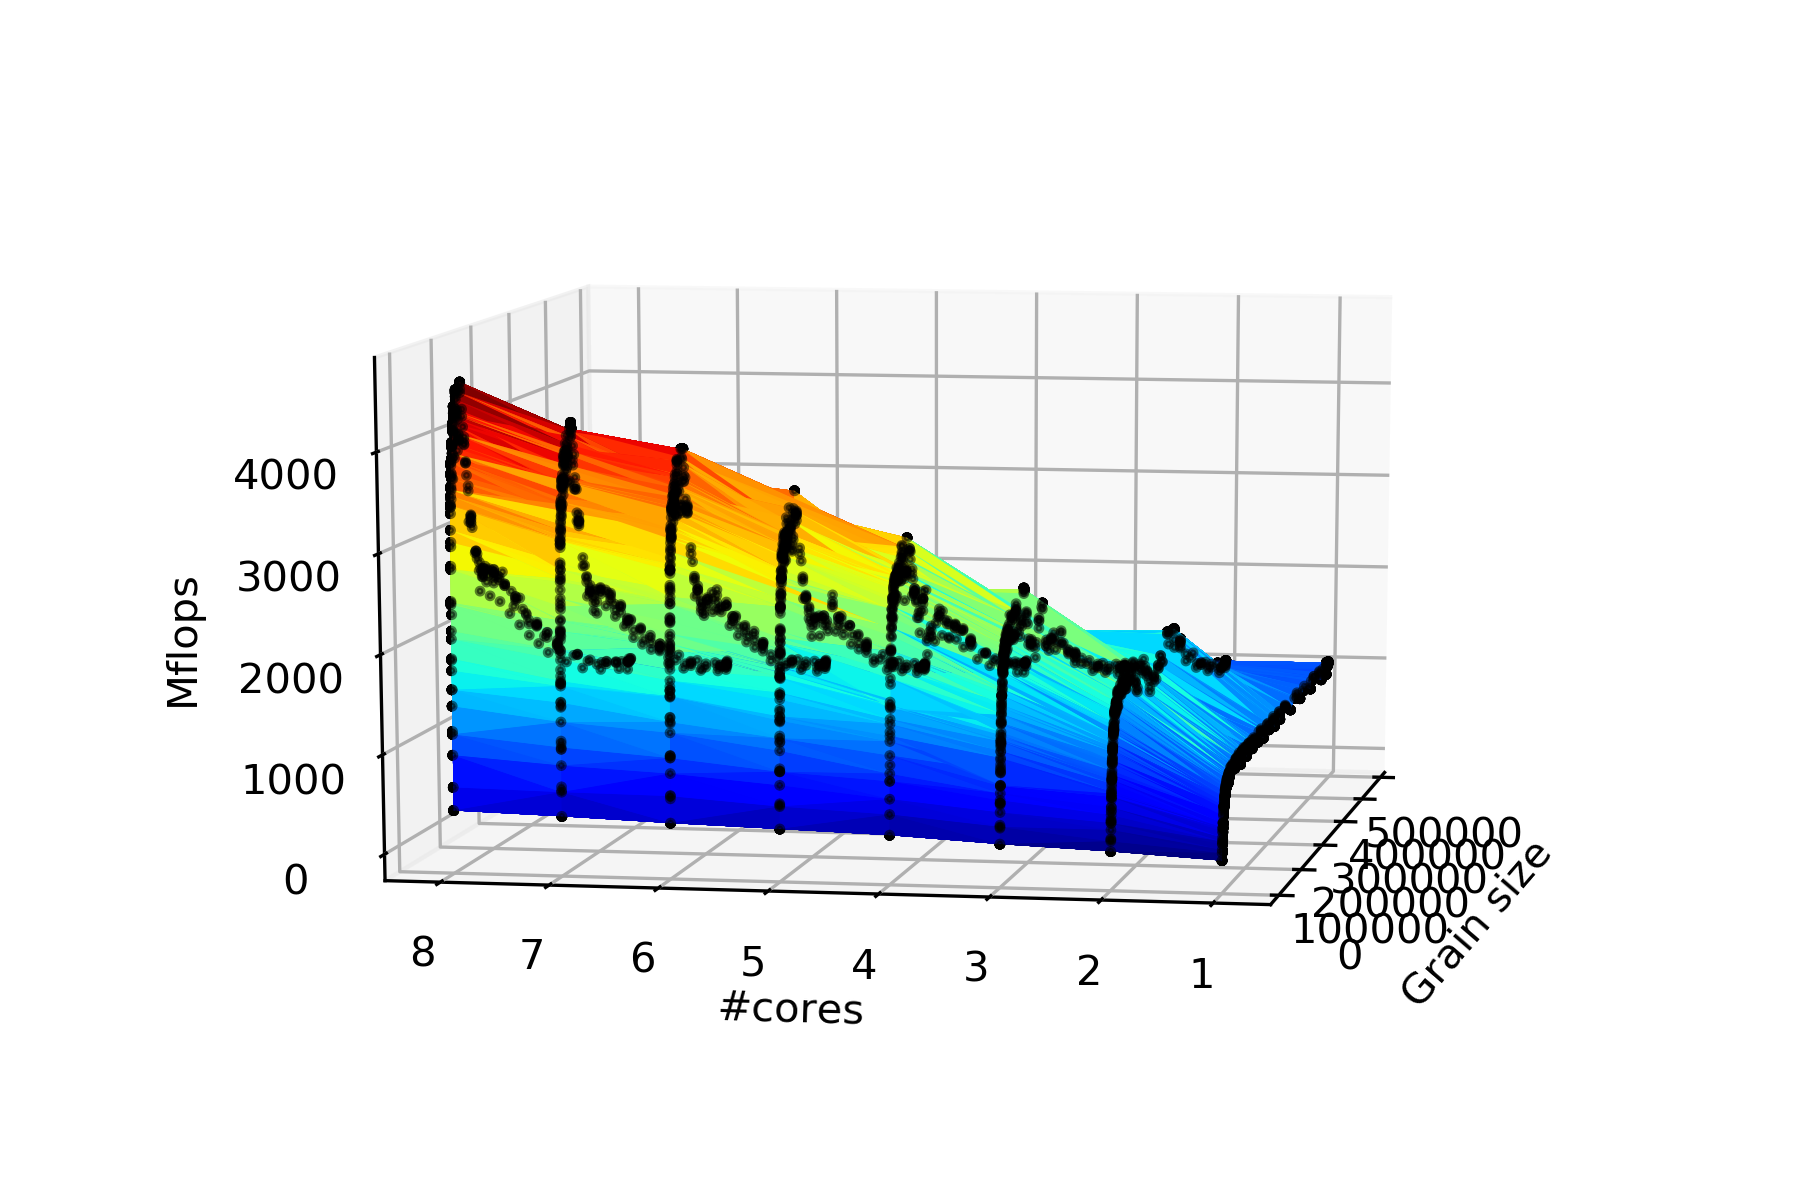
\includegraphics[width=1\linewidth]{images/fig3.png}
	\caption{An example of results obtained from Blazemark running $DMATDMATADD$ benchmark for matrix of size 690$\times$690 from two different angles}	
	\label{fig1}
\end{figure}

\subsection{Observation}

\subsection{L2 cache miss analysis}
In this set of experiments we used the performance counters integrated into HPX to measure the cache miss rate for different grain\textunderscore sizes w

-grain\textunderscore size
